\subsection{Outcome definitions}
\label{subsec:outcome_definitions_d1}

To disentangle how outcomes are shaped by professional partners versus celebrity attributes, we model
judges' evaluations and inferred fan preferences as two distinct but related outcomes.
For comparability across seasons and weeks, we work with \emph{shares} rather than raw scores.
Let $A_{s,t}$ denote the active set in season $s$, week $t$.

\paragraph{Judges' outcome.}
Define the judges' score share
\begin{equation}
q^{J}_{i,t}=\frac{J_{i,t}}{\sum_{r\in A_{s,t}}J_{r,t}},
\end{equation}
and use a logit transform with a small $\epsilon$ for stability:
\begin{equation}
y^{J}_{i,t}=\log\frac{q^{J}_{i,t}+\epsilon}{1-q^{J}_{i,t}+\epsilon}.
\end{equation}

\paragraph{Fans' outcome.}
Let Task~A provide the inferred vote share $p_{i,t}$ (denoted $q^{V}_{i,t}$). We similarly define
\begin{equation}
y^{V}_{i,t}=\log\frac{p_{i,t}+\epsilon}{1-p_{i,t}+\epsilon}.
\end{equation}
We adopt share + logit for cross-season comparability and interpret coefficients on the log-odds scale.

\noindent\textbf{Elimination outcome.}
Define a weekly elimination indicator
\[
E_{i,t}=
\begin{cases}
1, & \text{if contestant $i$ is eliminated in week $t$,}\\
0, & \text{otherwise.}
\end{cases}
\]
This outcome links the two channels (judges' evaluations and inferred fan support) to realized competition survival.


\subsection{Modeling results: separating ``who judges reward'' vs.\ ``who fans support''}
\label{subsec:modeling_results_d1}

We fit two parallel mixed-effects models, one for judges and one for fans, with shared covariates but distinct
random-effects structures. This allows us to quantify whether professional dancers act primarily as
(i) performance amplifiers in the judges' channel, (ii) popularity amplifiers in the fans' channel, or both.

\subsubsection{Model 1: Judges' evaluation model}
\label{subsubsec:model1_judges}

We model judges' logit-share as
\begin{equation}
y^{J}_{i,t}=\beta_0 + X_i^\top\beta + f(t) + \mathrm{FE}_s + v_{d(i)} + u_{i} + \varepsilon^{J}_{i,t},
\end{equation}
where $X_i$ are celebrity attributes (e.g., age, industry), $f(t)$ captures week effects,
$\mathrm{FE}_s$ are season fixed effects, $v_{d(i)}$ is a random intercept for the professional dancer partnered with celebrity $i$,
and $u_i$ is a contestant random effect capturing persistent idiosyncrasy.
The variance component $\sigma_v^2$ represents the professional-dancer effect on judges' evaluations.

\paragraph{Hypothesis test.}
A key hypothesis test is $H_0:\sigma_v^2=0$ (no pro-dancer effect on judges).

\subsubsection{Model 2: Fans' preference model}
\label{subsubsec:model2_fans}

We model fans' logit-share as
\begin{equation}
y^{V}_{i,t}=\gamma_0 + X_i^\top\gamma + f(t) + \mathrm{FE}_s + b_{d(i)} + u_i + \varepsilon^{V}_{i,t},
\end{equation}
where $b_{d(i)}$ captures the professional-dancer effect on fan preferences.
This is structurally parallel to Model 1, enabling a direct comparison of variance components and attribute coefficients.

\paragraph{Bridging judges to fans.}
To test whether judges' evaluations transmit to fan support, we also fit an augmented specification:
\begin{equation}
y^{V}_{i,t}=\gamma_0 + \gamma_J y^{J}_{i,t} + X_i^\top\gamma + f(t) + \mathrm{FE}_s + b_{d(i)} + u_i + \varepsilon^{V}_{i,t}.
\end{equation}
The coefficient $\gamma_J$ measures the transmission strength from judges to fans.

\subsubsection{Attribute preference gaps: judges vs.\ fans}
\label{subsubsec:attribute_gaps}

To quantify whether fans and judges value celebrity attributes differently, we compare the attribute coefficients across the two channels.
Let $\beta_k$ and $\gamma_k$ denote the coefficient on attribute $k$ in Models 1 and 2. Define the preference gap
\begin{equation}
\Delta_k=\gamma_k-\beta_k.
\end{equation}
$\Delta_k>0$ indicates fans prefer the attribute more than judges do; $\Delta_k<0$ indicates the opposite.
We report $\Delta_k$ with uncertainty bands (via bootstrap) whenever vote inference uncertainty is non-negligible.

\paragraph{Model 3: Elimination risk (competition outcome).}
To connect both channels to realized outcomes, we fit a discrete-time survival model for weekly elimination:
\[
\Pr(E_{i,t}=1)
=
\operatorname{logit}^{-1}\!\Big(
\theta_0
+\theta_J y^J_{i,t}
+\theta_V y^V_{i,t}
+\theta^\top X_i
+f(t)
+\mathrm{FE}_s
+r_{d(i)}
\Big),
\]
where $E_{i,t}$ is the elimination indicator from Section~\ref{subsec:outcome_definitions_d1}, and $r_{d(i)}$ captures professional-dancer heterogeneity in outcome risk.
This model quantifies how judges' evaluations, inferred fan support, and observed attributes jointly translate into elimination probability.


\paragraph{Quantifying professional-dancer impact (magnitude, not just significance).}
We quantify the fraction of outcome variance attributable to professional dancers using ICC-style ratios:
\begin{equation}
ICC^{J}_{pro}=\frac{\sigma_v^{2}}{\sigma_v^{2}+\sigma_u^{2}+\sigma^{2}},\qquad
ICC^{V}_{pro}=\frac{\sigma_b^{2}}{\sigma_b^{2}+\sigma_u^{2}+\sigma^{2}},
\end{equation}
where $\sigma_v^2$ is the variance of $v_{d(i)}$, $\sigma_b^2$ is the variance of $b_{d(i)}$,
$\sigma_u^2$ is the contestant-level variance, and $\sigma^2$ is the residual variance.
These ratios provide an interpretable measure of how much professional partners matter relative to persistent celebrity idiosyncrasy.

\subsubsection{Uncertainty propagation from vote inference}
\label{subsubsec:uncertainty_propagation_d1}

Because $p_{i,t}$ is inferred rather than observed, we propagate vote-inference uncertainty into downstream coefficients.
We do so either by (i) bootstrap resampling of the inference stage and re-fitting Models 2--3, or (ii) weighted regression using the interval width from Task A as an uncertainty proxy; we report confidence intervals accordingly.
In the weighted specification, let $w_{i,t}$ denote the feasible vote-interval width from Task A (KPI2).
We set observation weights
\[
\omega_{i,t}=\frac{1}{w_{i,t}+\varepsilon},
\]
so that more identifiable (tighter-interval) weeks exert greater influence, while poorly identified weeks are down-weighted rather than discarded.


\subsection{Impact of Dancers and Celebrities on Outcomes}
\subsubsection{Dancer Effects}
We first fix celebrities with comparable conditions and compare the differences in final rankings and scores across pairings with different dancers. Using the quantitative linear calculation method introduced earlier, 
we then compare the ICC values of different dancers and find that variations in dancers significantly affect final rankings. 
\begin{figure}[!htbp]
    \centering
    % 子图1：不同舞者对最终排名的影响
    \begin{subfigure}{0.48\textwidth}  % 调整子图宽度为页面48%，适配双列排版
        \centering
        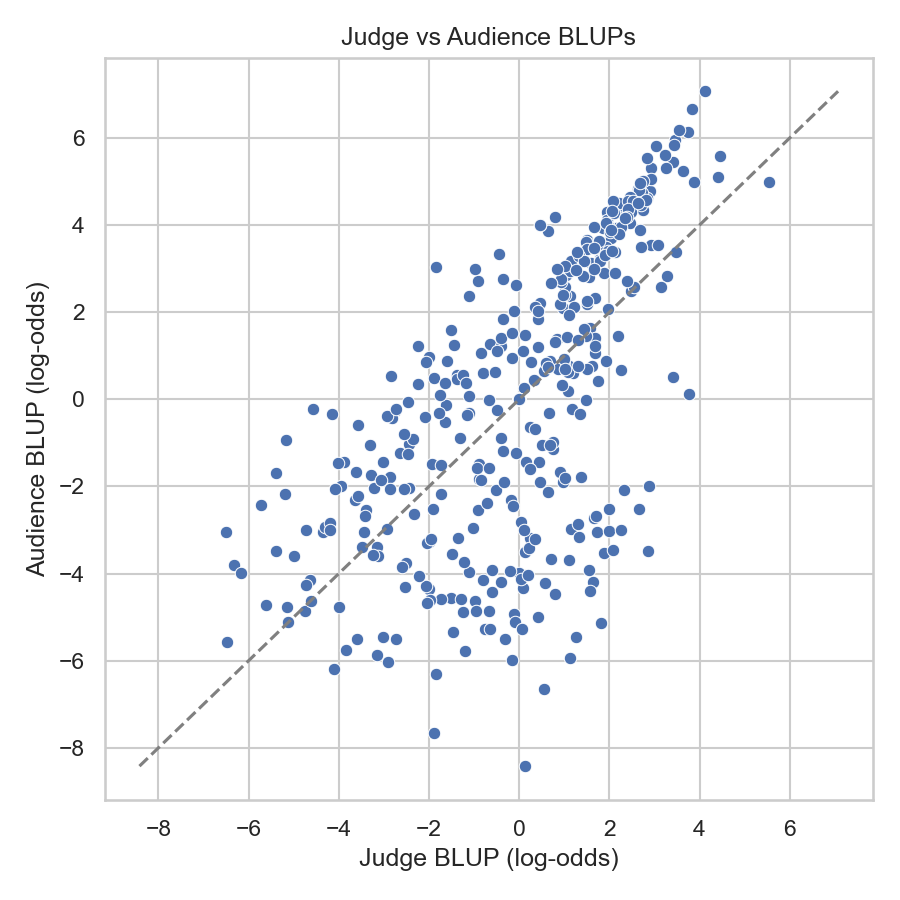
\includegraphics[width=0.95\linewidth]{output/fig/task3/cooperate_influence.png}
        \caption{Influence of different dancers on final rankings.}
        \label{fig:dancer_influence}
    \end{subfigure}
    \hfill  % 子图间自动填充空白（比 \quad 更适配双列）
    % 子图2：明星年龄对最终排名的影响
    \begin{subfigure}{0.48\textwidth}
        \centering
        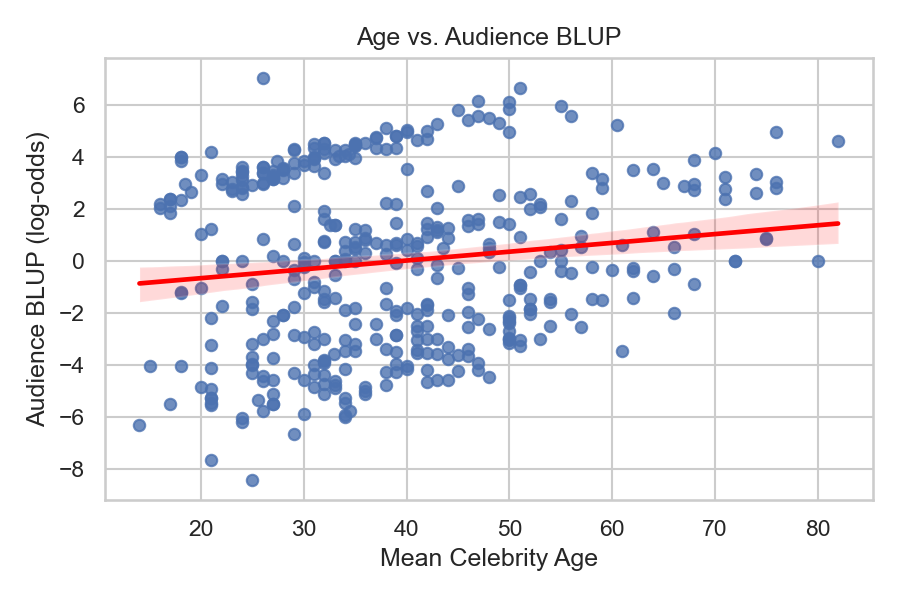
\includegraphics[width=0.95\linewidth]{output/fig/task3/age_influence.png}
        \caption{Influence of celebrity age on final rankings.}
        \label{fig:age_influence}
    \end{subfigure}
    
    % 总图标题（概括所有子图核心内容）
    \caption{Impacts of Dancer and Celebrity Age on Competition Final Rankings}
    % 总图标签（用于全文引用）
    \label{fig:rankings_influence}
\end{figure}
Such differences are practically attributed to a series of factors including experience and age; however, 
due to the lack of corresponding supporting data in the provided dataset, we do not conduct an in-depth analysis thereof.
\subsection{Impact of Celebrity Characteristics}
We calculate the trait preferences for relevant indicators of celebrities and obtain statistically significant results. Herein, we select age, industry, and other factors of celebrities for analysis.
\paragraph{Age}

In Tabel~\ref{fig:age_influence}, we find that older celebrities exhibit a stronger tendency to receive fan votes. That may be because older celebrities have a more established fan base and greater social influence, leading to higher vote counts.

\paragraph{Industry}
\begin{figure}[H]
    \centering
    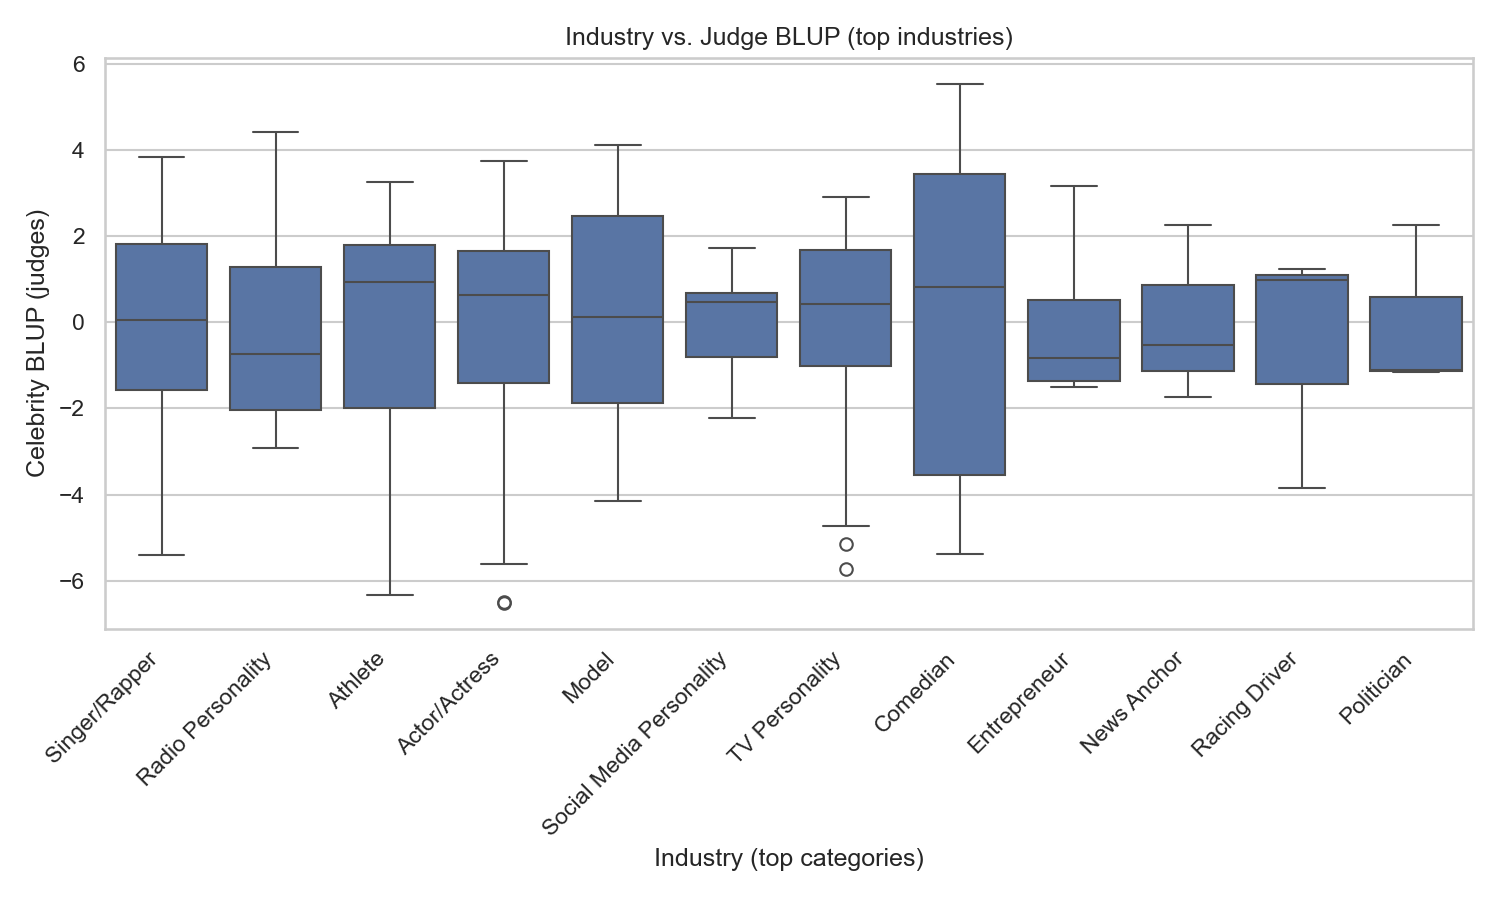
\includegraphics[width=0.95\linewidth]{output/fig/task3/industry_influence.png}
    \caption{Influence of celebrity industry on final rankings.}
    \label{fig:industry_influence}
\end{figure}
We find that different industries have a significant impact on final rankings. Among these, industries listed in Table~\ref{fig:industry_influence}, exert a significant positive effect on overall performance, while others tend to have less positive effect on overall performance.
\paragraph{Other Factors}
Differences in factors such as a celebrity's personal influence, dance foundation, and learning ability do exist and exert an impact in real scenarios. Thus, we argue that celebrities with greater personal influence, a solid dance foundation, and strong learning ability tend to achieve better performance. Nevertheless, these factors cannot be identified in the current dataset, and therefore we do not provide a quantitative interpretation thereof.


% ---------------- Figure/Table placeholders (insert later) ----------------
% Fig 6.1 Coefficient comparison (beta vs gamma) for key attributes.
% Fig 6.2 Preference gaps Delta_k with CI (bootstrap).
% Tab 6.1 ICC^{J}_{pro} and ICC^{V}_{pro} (overall + by era if desired).
% Tab 6.2 Top/bottom 5 pros by BLUP for judges and fans (side-by-side).
% ------------------------------------------------------------------------

% ======================================================================
% Chapter 6 Figures/Tables Placeholders (to be filled after model runs)
% Place this block at the END of:
%   6_impact_analysis_task_d1_pro_dancer_and_attributes.tex
% ======================================================================

% -----------------------------
% What MUST be backed by outputs (writing guardrails)
% -----------------------------
% Any claim of the form:
%   - "fans prefer X more than judges" / "judges reward X more"
%   - "gamma_J is significant/strong/weak"
%   - "pro dancer effect is large/non-negligible"
%   - "top/bottom pro dancer rankings"
% MUST be supported by the corresponding figure/table below.
% Otherwise hedge language: "we quantify / we evaluate / we report".

% % ======================================================================
% % FIGURE 6.1  Coefficient comparison (Judges vs Fans): beta_k vs gamma_k
% % ======================================================================
% % Purpose (MCM): show, at a glance, whether each attribute pushes judges and fans
% % in the same direction and with similar magnitude.
% % Inputs: model6_judge_coeffs.csv (beta, CI); model6_vote_coeffs.csv (gamma, CI)
% % Recommended: horizontal dot/interval plot, one row per feature, two series.
% % Insert in text: after the paragraph introducing the two models (Section 6.2).
% \begin{figure}[H]
%     \centering
%     %\includegraphics[width=0.95\linewidth]{figures/fig6_1_coef_compare.pdf}
%     \fbox{\parbox{0.95\linewidth}{\centering Placeholder: Fig 6.1 Coefficient comparison ($\beta_k$ vs $\gamma_k$)}}
%     \caption{Attribute effects in the Judge Model ($\beta_k$) versus the Vote Model ($\gamma_k$) on the log-odds scale (with 95\% confidence intervals).}
%     \label{fig:coef_compare_beta_gamma}
% \end{figure}

% % ======================================================================
% % FIGURE 6.2  Preference gap: Delta_k = gamma_k - beta_k (with uncertainty)
% % ======================================================================
% % Purpose (MCM): directly answers "who values what more" and supports any
% % narrative about preference differences.
% % Inputs: computed Delta_k table with CI from bootstrap or uncertainty propagation.
% % Insert in text: immediately after Fig 6.1 and the definition of Delta_k.
% \begin{figure}[H]
%     \centering
%     %\includegraphics[width=0.90\linewidth]{figures/fig6_2_delta_ci.pdf}
%     \fbox{\parbox{0.90\linewidth}{\centering Placeholder: Fig 6.2 Preference gaps ($\Delta_k$) with CI}}
%     \caption{Preference gaps $\Delta_k=\gamma_k-\beta_k$ for shared attributes. Positive values indicate stronger fan preference than judges; negative values indicate stronger judge preference (95\% confidence intervals via uncertainty propagation).}
%     \label{fig:delta_k_ci}
% \end{figure}

% % ======================================================================
% % TABLE 6.1  Variance components and ICC for pro-dancer effects
% % ======================================================================
% % Purpose (MCM): quantify magnitude (not just significance) of pro-dancer impact
% % on judges and fans. Supports statements like "pro accounts for X% variance".
% % Inputs: model6_variance_components.csv; compute ICC^J_pro and ICC^V_pro.
% % Insert in text: in Section 6.2 paragraph "Quantifying pro-dancer impact".
% \begin{table}[H]
%     \centering
%     %\input{tables/tab6_1_icc.tex}
%     \caption{Variance components and ICC-style ratios quantifying professional-dancer influence on judges' scores and inferred fan votes.}
%     \label{tab:icc_pro_effect}
% \end{table}

% % ======================================================================
% % TABLE 6.2  Pro-dancer BLUP rankings (Judges vs Fans), Top/Bottom 5
% % ======================================================================
% % Purpose (MCM): interpretable ranking of pros; supports case narratives and memo.
% % Inputs: BLUP random effects from Judge Model (v_pro) and Vote Model (b_pro).
% % Insert in text: after discussing BLUP interpretation and ICC results.
% \begin{table}[H]
%     \centering
%     %\input{tables/tab6_2_blup_top_bottom.tex}
%     \caption{Top and bottom professional dancers by fitted random effects (BLUPs), shown separately for judges' scores and inferred fan votes. Rankings are descriptive summaries of the fitted models.}
%     \label{tab:blup_pro_rankings}
% \end{table}

% % ======================================================================
% % OPTIONAL FIGURE 6.3  Transmission strength gamma_J (robustness / bootstrap)
% % ======================================================================
% % Purpose (MCM): make the "judges -> fans" transmission interpretable and robust.
% % Inputs: bootstrap_gamma_summary.csv (distribution of gamma_J across bootstrap runs)
% % Insert in text: after interpreting gamma_J in Vote Model.
% \begin{figure}[H]
%     \centering
%     %\includegraphics[width=0.75\linewidth]{figures/fig6_3_gammaJ_bootstrap.pdf}
%     \fbox{\parbox{0.75\linewidth}{\centering Optional: Fig 6.3 Bootstrap distribution of $\gamma_J$}}
%     \caption{Bootstrap distribution of the transmission coefficient $\gamma_J$ linking judges' evaluations to inferred fan votes.}
%     \label{fig:gammaJ_bootstrap}
% \end{figure}

% % ======================================================================
% % OPTIONAL TABLE 6.3  Model specification checklist (for reproducibility)
% % ======================================================================
% % Purpose (MCM): a compact audit table (FE, RE, trend, uncertainty method).
% % Insert in appendix if page-limited; keep here as optional.
% \begin{table}[H]
%     \centering
%     %\input{tables/tab6_3_model_spec_checklist.tex}
%     \caption{(Optional) Specification checklist for the Judge Model and Vote Model (fixed effects, random effects, week trend, season FE, and uncertainty propagation choice).}
%     \label{tab:model_spec_checklist}
% \end{table}

% % ======================================================================
% % Notes for the team (implementation mapping)
% % ======================================================================
% % Required artifacts to generate:
% % - figures/fig6_1_coef_compare.pdf  (beta vs gamma with CI)
% % - figures/fig6_2_delta_ci.pdf      (Delta_k with CI)
% % - tables/tab6_1_icc.tex            (variance components + ICC)
% % - tables/tab6_2_blup_top_bottom.tex (BLUP top/bottom 5)
% % Optional:
% % - figures/fig6_3_gammaJ_bootstrap.pdf
% % - tables/tab6_3_model_spec_checklist.tex
% % ======================================================================
